\subsection{切锥}\label{sec:7.3}\index{tangent cone@切锥（tangent cone）|hyperpage}
测地空间先验上没有可微结构，但可以为其构造替代物. 起点是角（angle）的概念：与曲率界的定义类似，可仿照 Hilbert 空间，在任意度量空间上定义角. 在测地空间中，角使我们能够定义方向，可将方向理解为常速测地线的初速度. 这些方向的集合构成切锥.

\subsubsection{角}\label{sec:7.3.1}
先在度量空间上定义角，并说明它给出了测地空间曲率界的其他刻画.

回顾，对任意三点 $p,x,y\in\mathbb R^2$，向量 $\overrightarrow{px}$ 与 $\overrightarrow{py}$ 形成的角 $\measuredangle_p(x,y)$ 的余弦为
$$\cos\measuredangle_p(x,y)=\frac{\langle x-p,y-p\rangle}{\lVert x-p\rVert\lVert y-p\rVert}.$$
注意
$$\begin{aligned}
-2\langle x-p,y-p\rangle
&=\lVert(x-p)-(y-p)\rVert^2-\lVert x-p\rVert^2-\lVert y-p\rVert^2\\
&=\lVert x-y\rVert^2-\lVert x-p\rVert^2-\lVert y-p\rVert^2.
\end{aligned}$$
因而可将定义改写为仅涉及距离平方的形式：
$$\cos\measuredangle_p(x,y)=\frac{\lVert x-p\rVert^2+\lVert y-p\rVert^2-\lVert x-y\rVert^2}{2\lVert x-p\rVert\lVert y-p\rVert}.$$
这个定义可以推广到任意度量空间.
\begin{definition}\label{def:7.16}
设 $(S,\mathsf d)$ 为度量空间. 对 $S$ 中任意三角形 $\{p,x,y\}$，通过下式定义 $p$ 处的角 $\measuredangle_p(x,y)\in[0,\pi]$：
$$\cos\measuredangle_p(x,y):=\frac{\mathsf d^2(p,x)+\mathsf d^2(p,y)-\mathsf d^2(x,y)}{2\mathsf d(p,x)\mathsf d(p,y)}.$$
\end{definition}
也可以与 $\kappa\ne0$ 的模型空间 $M_\kappa$ 进行类似比较，但这超出了本讲义的范围.

下一个结果用角的单调性刻画正曲率空间.
\begin{proposition}[角的单调性]\label{prop:7.17}
设 $(S,\mathsf d)$ 为测地空间. 则\autoref{def:7.9}意义下的 $\operatorname{curv}(S)\ge0$ 成立，当且仅当对 $S$ 中任意三角形 $\{p,x,y\}$ 及分别连接 $p$ 与 $x$、$p$ 与 $y$ 的任意测地线 $\omega,\omega'$，函数
$$(s,t)\in[0,1]^2\mapsto\measuredangle_p(\omega(s),\omega'(t))$$
在固定其中一个变量时，关于另一个变量单调不增.
\end{proposition}
\begin{proof}
先假设 $\operatorname{curv}(S)\ge0$，考虑 $S$ 中三角形 $\{p,x,y\}$ 及分别连接 $p$ 与 $x$、$p$ 与 $y$ 的常速测地线 $\omega,\omega'$. 只需证明对所有 $(s,t)\in[0,1]^2$ 有
$$\cos\measuredangle_p(\omega(s),\omega'(t))\le\cos\measuredangle_p(x,y).$$
令 $\{\bar p,\bar x,\bar y\}$ 为 $M_0=\mathbb R^2$ 中的比较三角形，$\bar\omega,\bar\omega'$ 为 $M_0$ 中分别连接 $\bar p$ 与 $\bar x$、$\bar p$ 与 $\bar y$ 的常速测地线. 则
$$\begin{aligned}
&\cos\measuredangle_p(\omega(s),\omega'(t))\\
&=\frac{\mathsf d^2(p,\omega(s))+\mathsf d^2(p,\omega'(t))-\mathsf d^2(\omega(s),\omega'(t))}{2\mathsf d(p,\omega(s))\mathsf d(p,\omega'(t))}\\
&=\frac{s^2\mathsf d^2(p,x)+t^2\mathsf d^2(p,y)-\mathsf d^2(\omega(s),\omega'(t))}{2st\mathsf d(p,x)\mathsf d(p,y)}\\
&=\frac{s^2\lVert\bar p-\bar x\rVert^2+t^2\lVert\bar p-\bar y\rVert^2-\mathsf d^2(\omega(s),\omega'(t))}{2st\lVert\bar p-\bar x\rVert\lVert\bar p-\bar y\rVert}\\
&\le\frac{s^2\lVert\bar p-\bar x\rVert^2+t^2\lVert\bar p-\bar y\rVert^2-\lVert\bar\omega(s)-\bar\omega'(t)\rVert^2}{2st\lVert\bar p-\bar x\rVert\lVert\bar p-\bar y\rVert}\\
&=\frac{\lVert\bar p-\bar\omega(s)\rVert^2+\lVert\bar p-\bar\omega'(t)\rVert^2-\lVert\bar\omega(s)-\bar\omega'(t)\rVert^2}{2\lVert\bar p-\bar\omega(s)\rVert\lVert\bar p-\bar\omega'(t)\rVert}\\
&=\cos\measuredangle_{\bar p}(\bar\omega(s),\bar\omega'(t))
=\cos\measuredangle_{\bar p}(\bar x,\bar y)=\cos\measuredangle_p(x,y),
\end{aligned}$$
其中不等式使用 $\operatorname{curv}(S)\ge0$ 和\autoref{prop:7.13}. 曲率下界蕴含角的单调性得证.

反之，假设对 $S$ 中任意三角形 $\{p,x,y\}$、分别连接 $p$ 与 $x$、$p$ 与 $y$ 的任意常速测地线 $\omega,\omega'$ 以及所有 $(s,t)\in[0,1]^2$，有
$$\cos\measuredangle_p(\omega(s),\omega'(t))\le\cos\measuredangle_p(x,y).$$
那么，由证明的第一部分可知，在上述记号下有
$$\mathsf d^2(\omega(s),\omega'(t))\ge\lVert\bar\omega(s)-\bar\omega'(t)\rVert^2,\qquad\forall(s,t)\in[0,1]^2,$$
这正是\autoref{prop:7.13}中 $\operatorname{curv}(S)\ge0$ 的刻画.
\end{proof}

\subsubsection{方向}\label{sec:7.3.2}
由点之间的角，可以直接定义常速测地线之间的角.

设 $(S,\mathsf d)$ 是满足 $\operatorname{curv}(S)\ge0$ 的测地空间，$p\in S$，$\omega,\omega'$ 分别是连接 $p$ 与 $x$、$p$ 与 $y$ 的常速测地线. 定义它们之间的角为
$$\measuredangle(\omega,\omega'):=\lim_{s,t\searrow0}\measuredangle_p(\omega(s),\omega'(t)).$$
由\autoref{prop:7.17}，在 $\operatorname{curv}(S)\ge0$ 的假设下，该极限存在. 事实上，在同一假设下还有
$$\measuredangle(\omega,\omega')=\lim_{t\searrow0}\measuredangle_p(\omega(t),\omega'(t)).$$
给定第三条常速测地线 $\omega'':[0,1]\to S$，满足 $\omega''(0)=p$、$\omega''(1)=z$，可以证明（见\autoref{exer:7.4}）下述三角不等式：
\begin{equation}\label{eq:7.12}
\measuredangle(\omega,\omega')\le\measuredangle(\omega,\omega'')+\measuredangle(\omega'',\omega'),
\end{equation}
所以 $\measuredangle$ 是从 $p$ 出发的所有常速测地线集合 $\mathcal G(p)$ 上的伪度量. 接着在 $\mathcal G(p)$ 上定义等价关系 $\sim$：
$$\omega\sim\omega'\quad\Longleftrightarrow\quad\measuredangle(\omega,\omega')=0.$$
在商集 $\mathcal G(p)/{\sim}$ 上，$\measuredangle$ 成为真正的度量，仍记为 $\measuredangle$.
\begin{definition}\label{def:7.18}
从 $p$ 出发的方向空间（space of directions）是 $(\mathcal G(p)/{\sim},\measuredangle)$ 的完备化 $(\Sigma_p,\measuredangle)$. $\Sigma_p$ 中的元素称为方向（direction）.
\end{definition}

\subsubsection{切锥}\label{sec:7.3.3}
切锥的概念为测地空间提供了切空间的类似物.
\begin{definition}[切锥]\label{def:7.19}\index{tangent cone@切锥（tangent cone）|hyperpage}
设 $(S,\mathsf d)$ 为具有正曲率的测地空间，固定 $p\in S$. $p$ 处的切锥（tangent cone）$T_pS$ 是方向空间 $(\Sigma_p,\measuredangle)$ 上的欧氏锥. 换言之，$T_pS$ 是如下度量空间：
\begin{itemize}
\item 其底层集合由 $\Sigma_p\times[0,+\infty)$ 在下述等价关系下的等价类组成：
$$(\omega,s)\sim(\omega',t)\quad\Longleftrightarrow\quad
\begin{cases}s=t=0,\\\text{或 }\omega=\omega'\text{ 且 }s=t;\end{cases}$$
\item 其度量 $\mathsf d_p$ 定义为
$$\mathsf d_p((\omega,s),(\omega',t)):=\sqrt{s^2+t^2-2st\cos\measuredangle(\omega,\omega')}.$$
\end{itemize}
\end{definition}
对 $u=(\omega,s)$ 与 $v=(\omega',t)\in T_pS$，记 $\lVert u-v\rVert_p:=\mathsf d_p(u,v)$、$\lVert u\rVert_p:=\mathsf d_p(o_p,u)$，其中 $o_p=(\omega,0)\in T_pS$ 是锥顶，并记
$$\langle u,v\rangle_p:=\lVert u\rVert_p\lVert v\rVert_p\cos\measuredangle(\omega,\omega')
=\frac12(\lVert u\rVert_p^2+\lVert v\rVert_p^2-\lVert u-v\rVert_p^2).$$
之所以使用“锥”这个名称以及上述记号 $\lVert\cdot\rVert_p$、$\langle\cdot,\cdot\rangle_p$，是因为锥 $T_pS$ 具有下述类似 Hilbert 空间的结构. 度量几何中常见的做法是，仅使用测地空间上存在的概念，将欧氏概念重新表达；$\mathsf d_p$ 的定义正是如此，这里用到的是距离与角. 事实上，若 $\omega,\omega'$ 是球面上的点，并将 $(\omega,s):=s\cdot\omega$、$(\omega',t):=t\cdot\omega'$，则由余弦定理，两者的距离平方为
\begin{equation}\label{eq:7.13}
\lVert s\cdot\omega-t\cdot\omega'\rVert^2=s^2+t^2-2st\cos\measuredangle(\omega,\omega').
\end{equation}
对点 $u=(\omega,t)$ 和 $\lambda\ge0$，定义 $\lambda\cdot u:=(\omega,\lambda t)$. 此外，由上述定义可验证，对任意 $u,v\in T_pS$ 与 $\lambda\ge0$，有
$$\lVert\lambda\cdot u\rVert_p=\lambda\lVert u\rVert_p,
\qquad\langle\lambda\cdot u,v\rangle_p=\langle u,\lambda\cdot v\rangle_p=\lambda\langle u,v\rangle_p.$$
注意，切锥可能不是测地的；但若它是测地的，则点 $u,v\in T_pS$ 的和定义为 $2\cdot u$ 与 $2\cdot v$ 的中点，如\hyperref[prop:7.5]{定义 7.5}所定义. 在这种情形下，$T_pS$ 确实是一个锥.

一个值得记住的例子是，$S$ 为平面 $\mathbb R^2$ 中填满内部的正方形. 在 $S$ 的某个顶点处，切锥“缺少”某些方向，即那些会走出 $S$ 的方向，所以不是向量空间；这就是不称它为切“空间”的原因.

对数映射将在后文起重要作用. 对所有 $x\in S$，用 $\Uparrow_p^x\subset\Sigma_p$ 表示 $S$ 中连接 $p$ 与 $x$ 的所有常速测地线的等价类集合. 然后，对每个 $x\in S$，任意选取一个方向 $\uparrow_p^x\in\Uparrow_p^x$.
\begin{definition}[对数映射]\label{def:7.20}\index{logarithmic map@对数映射（logarithmic map）|hyperpage}
设 $(S,\mathsf d)$ 为正曲率测地空间. 对每个 $x\in S$ 选定 $\uparrow_p^x\in\Uparrow_p^x$ 后，相应的对数映射（logarithmic map）定义为
$$\log_p:x\in S\mapsto(\uparrow_p^x,\mathsf d(p,x))\in T_pS.$$
\end{definition}
在这种一般性下，$\log_p(x)$ 的定义依赖方向的选择 $\{\uparrow_p^x,x\in S\}$. 将 $\log_p$ 限制在适当子集上，就能消除歧义：即那些连接 $p$ 与 $x$ 的常速测地线只有一个方向等价类的点 $x\in S$. 还可以更精确地说明这一集合：在 NNC 空间 $S$ 中，若从 $p$ 到 $x$ 的常速测地线 $\omega,\omega'$ 满足 $\measuredangle(\omega,\omega')=0$，则 $\omega=\omega'$. 换言之，连接 $p$ 与 $x$ 的常速测地线有不止一个等价类的点集，恰是与 $p$ 至少由两条不同常速测地线相连的点集. 该集合记为 $C(p)$，称为 $p$ 的割迹（cut-locus）. 对任意 $x\in S\setminus C(p)$，$\log_p(x)$ 无歧义地定义为
$$\log_p(x)=(\omega_x,\mathsf d(p,x)),$$
其中 $\omega_x$ 是从 $p$ 到 $x$ 的唯一常速测地线，因此与其方向等同. 特别地，在此记号下，对所有 $t\in[0,1]$ 与 $x\in S\setminus C(p)$，有
$$\log_p\omega_x(t)=t\log_px.$$
更一般地，若 $\omega:[0,1]\to S$ 是 $S$ 中的常速测地线，且对某个 $t\in[0,1]$ 有 $p=\omega(t)$，即 $p$ 位于该测地线上，则
\begin{equation}\label{eq:7.14}
\log_p\omega(s)=(1-s)\log_p\omega(0)+s\log_p\omega(1).
\end{equation}
换言之，对数映射将测地线变成直线.

下述结果说明，$\log_p$ 映射在正曲率空间中是扩张的.
\begin{proposition}\label{prop:7.21}
设 $(S,\mathsf d)$ 是测地空间，固定 $p\in S$. 若 $\operatorname{curv}(S)\ge0$，则对数映射在如下意义下是扩张的：对所有 $x,y\in S$，有
$$\mathsf d(x,y)\le\lVert\log_p(x)-\log_p(y)\rVert_p,$$
且当 $x=p$ 或 $y=p$ 时取等号.
\end{proposition}
\begin{proof}
设 $\omega,\omega'$ 分别是连接 $p$ 与 $x$、$p$ 与 $y$ 的两条常速测地线. 若 $p\ne x$ 且 $p\ne y$，根据 $\lVert\cdot\rVert_p$ 的定义和角的单调性，对所有 $s,t\in[0,1]$ 有
$$\begin{aligned}
\lVert\log_p(x)-\log_p(y)\rVert_p^2
&=\mathsf d_p^2(\log_p(x),\log_p(y))\\
&=\mathsf d^2(p,x)+\mathsf d^2(p,y)-2\mathsf d(p,x)\mathsf d(p,y)\cos\measuredangle(\omega,\omega')\\
&\ge\mathsf d^2(p,x)+\mathsf d^2(p,y)-2\mathsf d(p,x)\mathsf d(p,y)\cos\measuredangle_p(\omega(s),\omega'(t)).
\end{aligned}$$
应用\autoref{def:7.16}，得到
$$\begin{aligned}
&\lVert\log_p(x)-\log_p(y)\rVert_p^2\\
&\ge\mathsf d^2(p,x)+\mathsf d^2(p,y)
-\frac{s^2\mathsf d^2(p,x)+t^2\mathsf d^2(p,y)-\mathsf d^2(\omega(s),\omega'(t))}{st}.
\end{aligned}$$
令 $s=t=1$，得到
$$\lVert\log_p(x)-\log_p(y)\rVert_p^2\ge\mathsf d^2(x,y).$$
等号情形容易由 $\mathsf d_p$ 的定义验证.
\end{proof}

\subsubsection{Wasserstein 空间的切锥}\label{sec:7.3.4}
从切锥定义本身出发，可以说明它在 Wasserstein 情形中具有非常简单的形式. 为此，令 $\mu,\nu,\rho\in\mathcal W_2$ 为三个概率分布，$\omega_\nu,\omega_\rho$ 分别是 $2$-Wasserstein 空间中连接 $\mu$ 与 $\nu$、$\mu$ 与 $\rho$ 的两条测地线. 回顾，$\mu$ 处的切锥是配备下述距离 $\mathsf d_\mu$ 的方向度量空间：
$$\begin{aligned}
&\mathsf d_\mu^2((\omega_\nu,\mathsf d(\mu,\nu)),(\omega_\rho,\mathsf d(\mu,\rho)))\\
&=W_2^2(\mu,\nu)+W_2^2(\mu,\rho)-2W_2(\mu,\nu)W_2(\mu,\rho)\cos\measuredangle(\omega_\nu,\omega_\rho).
\end{aligned}$$
这两条 Wasserstein 测地线间的角 $\measuredangle(\omega_\nu,\omega_\rho)$ 是什么？假设 $\mu$ 有密度，就能进行计算. 此时 Brenier 定理保证两个最优传输映射 $T_{\mu\to\nu}$ 与 $T_{\mu\to\rho}$ 存在，因而
$$\begin{aligned}
\cos\measuredangle(\omega_\nu,\omega_\rho)
&=\lim_{t\searrow0}\frac{W_2^2(\mu,\omega_\nu(t))+W_2^2(\mu,\omega_\rho(t))-W_2^2(\omega_\nu(t),\omega_\rho(t))}{2W_2(\mu,\omega_\nu(t))W_2(\mu,\omega_\rho(t))}\\
&=\lim_{t\searrow0}\frac{t^2W_2^2(\mu,\nu)+t^2W_2^2(\mu,\rho)-W_2^2(\omega_\nu(t),\omega_\rho(t))}{2t^2W_2(\mu,\nu)W_2(\mu,\rho)}\\
&=\frac{W_2^2(\mu,\nu)+W_2^2(\mu,\rho)-\lim_{t\searrow0}\frac{W_2^2(\omega_\nu(t),\omega_\rho(t))}{t^2}}{2W_2(\mu,\rho)W_2(\mu,\nu)}.
\end{aligned}$$

\begin{lemma}\label{lem:7.22}
设 $\mu\in\mathcal P_{2,\mathrm{ac}}(\mathbb R^d)$，分别用 $T_{\mu\to\nu}$ 与 $T_{\mu\to\rho}$ 表示从 $\mu$ 到 $\nu$、从 $\mu$ 到 $\rho$ 的 Brenier 映射. 则
$$\lim_{t\searrow0}\frac{W_2^2(\omega_\nu(t),\omega_\rho(t))}{t^2}
=\lVert T_{\mu\to\nu}-T_{\mu\to\rho}\rVert_{L^2(\mu)}^2.$$
\end{lemma}
\begin{proof}
所需不等式中的一个方向容易证明. 令 $X\sim\mu$，注意
$$\begin{aligned}
X_t^\nu&:=(1-t)X+tT_{\mu\to\nu}(X)\sim\omega_\nu(t),\\
X_t^\rho&:=(1-t)X+tT_{\mu\to\rho}(X)\sim\omega_\rho(t).
\end{aligned}$$
所以
\begin{equation}\label{eq:7.15}
\begin{aligned}
W_2^2(\omega_\nu(t),\omega_\rho(t))&\le\mathbb E\lVert X_t^\nu-X_t^\rho\rVert^2\\
&=t^2\mathbb E\lVert T_{\mu\to\nu}(X)-T_{\mu\to\rho}(X)\rVert^2\\
&=t^2\lVert T_{\mu\to\nu}-T_{\mu\to\rho}\rVert_{L^2(\mu)}^2.
\end{aligned}
\end{equation}
为证明反方向，对任意 $t\in[0,1]$，令 $\Upsilon_t$ 是五个随机变量之间的如下耦合：当以下条件成立时，$(X,Y,Z,Y_t,Z_t)\sim\Upsilon_t$：
\begin{enumerate}
\item $X\sim\mu$ 与 $Y=T_{\mu\to\nu}(X)\sim\nu$ 最优耦合；
\item $Y_t=(1-t)X+tY\sim\omega_\nu(t)$；
\item $Z_t\sim\omega_\rho(t)$ 与 $Y_t\sim\omega_\nu(t)$ 最优耦合；
\item $Z_t\sim\omega_\rho(t)$ 与 $Z\sim\rho$ 最优耦合；
\item $Z_t\sim\omega_\rho(t)$ 与 $X'\sim\mu$ 最优耦合.
\end{enumerate}
\autoref{fig:7.1}表明，由于所得图无环，可以利用粘合引理实现这个联合耦合. 特别注意 $Z_t=(1-t)X'+tZ$. 有
\begin{equation}\label{eq:7.16}
\begin{aligned}
W_2^2(\omega_\nu(t),\omega_\rho(t))
&=\mathbb E\lVert Y_t-Z_t\rVert^2=\mathbb E\lVert(1-t)X+tY-Z_t\rVert^2\\
&=(1-t)\mathbb E\lVert X-Z_t\rVert^2+t\mathbb E\lVert Y-Z_t\rVert^2
-t(1-t)\mathbb E\lVert X-Y\rVert^2,
\end{aligned}
\end{equation}
\begin{figure}[htbp]
\centering
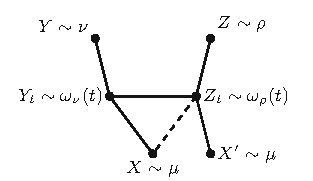
\includegraphics[width=0.65\linewidth]{assets/chapter7/fig7-1.pdf}
\caption{$(\mu,\nu,\rho,\omega_\nu(t),\omega_\rho(t))$ 之间的耦合 $\Upsilon_t$. 实线表示最优耦合；虚线与缺失的连线表示可能次优的耦合.}\label{fig:7.1}
\end{figure}
其中使用了 $\mathbf H=\mathbb R^d$ 时的\autoref{lem:7.10}. 现在注意，$X$ 与 $Z_t$ 的耦合可能次优，因此
$$(1-t)\mathbb E\lVert X-Z_t\rVert^2\ge(1-t)W_2^2(\mu,\omega_\rho(t))
=t^2(1-t)W_2^2(\mu,\rho).$$
此外，再次使用\autoref{lem:7.10}，得到
$$\begin{aligned}
t\mathbb E\lVert Y-Z_t\rVert^2
&=t\mathbb E\lVert Y-(1-t)X'+tZ\rVert^2\\
&=t(1-t)\mathbb E\lVert Y-X'\rVert^2+t^2\mathbb E\lVert Y-Z\rVert^2-t^2(1-t)\mathbb E\lVert X'-Z\rVert^2\\
&\ge t(1-t)\mathbb E\lVert Y-X\rVert^2+t^2\mathbb E\lVert Y-Z\rVert^2-t^2(1-t)\mathbb E\lVert X'-Z\rVert^2,
\end{aligned}$$
其中不等式使用 $X$ 与 $Y$ 最优耦合. 将以上两式代入 \eqref{eq:7.16}，可见含 $\mathbb E\lVert Y-X\rVert^2$ 的项抵消，得到
$$\begin{aligned}
W_2^2(\omega_\nu(t),\omega_\rho(t))
&\ge t^2(1-t)W_2^2(\mu,\rho)+t^2\mathbb E\lVert Y-Z\rVert^2-t^2(1-t)\mathbb E\lVert X'-Z\rVert^2\\
&=t^2\mathbb E\lVert Y-Z\rVert^2.
\end{aligned}$$
回顾 \eqref{eq:7.15}，有 $W_2(\omega_\nu(t),\omega_\rho(t))=O(t)$，故 $\mathbb E\lVert Y_t-Z_t\rVert^2=O(t^2)$. 由于
$$X=(Y_t-tY)/(1-t)\qquad\text{且}\qquad X'=(Z_t-tZ)/(1-t),$$
还可推出 $\mathbb E\lVert X-X'\rVert^2=O(t^2)$. 不加论证地假设 $T_{\mu\to\rho}$ 为 Lipschitz，\footnote{可通过逼近论证去掉这个假设，但需要额外的技术处理.} 则
$$\begin{aligned}
\mathbb E\lVert Y-Z\rVert^2
&=\mathbb E\lVert T_{\mu\to\nu}(X)-T_{\mu\to\rho}(X')\rVert^2\\
&=\mathbb E\lVert T_{\mu\to\nu}(X)-T_{\mu\to\rho}(X)\rVert^2-O(t).
\end{aligned}$$
由此立即得到
$$\lim_{t\searrow0}\frac{W_2^2(\omega_\nu(t),\omega_\rho(t))}{t^2}
\ge\lVert T_{\mu\to\nu}-T_{\mu\to\rho}\rVert_{L^2(\mu)}^2,$$
从而完成引理的证明.
\end{proof}

由\autoref{lem:7.22}，
\begin{equation}\label{eq:7.17}
\begin{aligned}
\cos\measuredangle(\omega_\nu,\omega_\rho)
&=\frac{W_2^2(\mu,\nu)+W_2^2(\mu,\rho)-\lVert T_{\mu\to\nu}-T_{\mu\to\rho}\rVert_{L^2(\mu)}^2}{2W_2(\mu,\nu)W_2(\mu,\rho)}\\
&=\frac{\lVert T_{\mu\to\nu}-\mathrm{id}\rVert_{L^2(\mu)}^2+\lVert T_{\mu\to\rho}-\mathrm{id}\rVert_{L^2(\mu)}^2-\lVert T_{\mu\to\nu}-T_{\mu\to\rho}\rVert_{L^2(\mu)}^2}{2\lVert T_{\mu\to\nu}-\mathrm{id}\rVert_{L^2(\mu)}\lVert T_{\mu\to\rho}-\mathrm{id}\rVert_{L^2(\mu)}}\\
&=\cos\measuredangle(T_{\mu\to\nu}-\mathrm{id},T_{\mu\to\rho}-\mathrm{id}),
\end{aligned}
\end{equation}
其中最后的余弦是在 Hilbert 空间 $L^2(\mu)$ 中理解的. 进而，余弦定理 \eqref{eq:7.13} 表明，$\mu$ 处切锥的度量为
$$\begin{aligned}
\mathsf d_\mu^2((\omega_\nu,s),(\omega_\rho,t))
&=s^2+t^2-2st\cos\measuredangle(\omega_\nu,\omega_\rho)\\
&=s^2+t^2-2st\cos\measuredangle(T_{\mu\to\nu}-\mathrm{id},T_{\mu\to\rho}-\mathrm{id})\\
&=\lVert s(T_{\mu\to\nu}-\mathrm{id})-t(T_{\mu\to\rho}-\mathrm{id})\rVert_{L^2(\mu)}^2.
\end{aligned}$$
因此，配备度量 $\mathsf d_\mu$ 的切锥与某个 Hilbert 空间等距. 我们已证明如下定理；\autoref{sec:5.4}用 Otto 微积分形式体系时，已经识别出这一结果.
\begin{theorem}\label{thm:7.23}
设 $\mu\in\mathcal P_{2,\mathrm{ac}}(\mathbb R^d)$. 则 $\mu$ 处的切锥 $T_\mu\mathcal W_2(\mathbb R^d)$ 是 $L^2(\mu)$ 的一个凸子集. 此外，对任意 $\nu\in\mathcal P_2(\mathbb R^d)$，有
$$\log_\mu(\nu)=T_{\mu\to\nu}-\mathrm{id}\in L^2(\mu),$$
其中 $T_{\mu\to\nu}$ 是从 $\mu$ 到 $\nu$ 的 Brenier 映射.
\end{theorem}
在上述情形中，配备\autoref{def:7.18}中 $\langle\cdot,\cdot\rangle$ 的切锥 $T_\mu\mathcal W_2$ 实际上是 Hilbert 空间的一个凸子集，我们略微滥用术语，称其为 $\mu$ 处的切空间（tangent space）. 从对数映射定义立即可知，对任意 $\nu,\rho\in\mathcal P_2(\mathbb R^d)$，内积 $\langle\cdot,\cdot\rangle_\mu$ 为
$$\begin{aligned}
\langle\log_\mu(\nu),\log_\mu(\rho)\rangle_\mu
&=\langle T_{\mu\to\nu}-\mathrm{id},T_{\mu\to\rho}-\mathrm{id}\rangle_{L^2(\mu)}\\
&=\int\langle T_{\mu\to\nu}(x)-x,T_{\mu\to\rho}(x)-x\rangle\,\mu(dx).
\end{aligned}$$
